\documentclass[a4paper,12pt]{article}
\usepackage{graphicx}
\usepackage{amsmath}
\usepackage{geometry}
\usepackage{longtable}
\usepackage{booktabs}

\title{Data Extraction, Preprocessing and Clustering Report:\\ EcoWheataly – Durum Wheat Dataset}
\author{EcoWheataly Team}
\date{\today}

\begin{document}

\maketitle

\section{Objective}

This report describes the construction of a clean, structured dataset from raw JSON data and the implementation of a clustering analysis pipeline on durum wheat farms in Italy. The final goal is to uncover meaningful farm-level typologies based on input use, costs, and productivity indicators, supporting simulation and policy evaluation in the EcoWheataly framework.

\section{Database and Extraction Process}

The input is a nested JSON file containing yearly farm-level information from 2008 to 2022. Each farm entry includes general data (like total farm acreage) and crop-specific details under the key \texttt{durum\_wheat}, such as production quantities, crop areas, labor and machinery costs, as well as fertilization and phytosanitary product usage.

The extraction process involves several steps. First, general agricultural and economic variables are collected: produced quantity, PLV, crop acreage, hours of machinery use, and different cost components. Then, fertilizer-related information is extracted and structured both at the aggregate level and broken down by type (Mineral, OrganoMineral, Other, Micro-Mineral). Each type contains specific details such as distribution area, nutrient content, and costs.

Phytosanitary products are extracted by category (Herbicide, Insecticide, Fungicide) and classified by toxicity levels (0–4). These quantities are aggregated per hectare and stored in structured arrays, later converted into a unified 2D dataset.

\section{Merging, Cleaning and Output Dataset}

All collected data are merged by farm and year into a single DataFrame. Missing values in phytosanitary products are interpreted as non-use and replaced with zeros. Other NaNs are flagged and addressed through filtering. Outliers such as infinite values (e.g., from division by zero) are also removed to ensure numerical consistency. Basic statistics per year are printed to assess coverage and integrity.

The result is a flattened, cleaned panel dataset saved as \texttt{flat\_df2.csv}, which serves as the input for machine learning and clustering tasks.

To further refine the dataset and mitigate the impact of extreme values, a robust outlier detection procedure was applied to a selected set of continuous numeric variables using an adjusted boxplot method. This approach extends the classic Tukey rule by incorporating an asymmetry correction based on the \textit{simplified medcouple}, a robust estimator of skewness. This allows for more reliable outlier identification in variables that exhibit significant skew.

The variables subjected to this cleaning step are:

\begin{itemize}
    \item \texttt{crop\_acreage}
    \item \texttt{produced\_quantity}
    \item \texttt{PLV} (Production value)
    \item \texttt{hours\_of\_machines\_ha}
    \item \texttt{fert\_costs}
    \item \texttt{phyto\_costs}
    \item \texttt{human\_costs}
    \item \texttt{thirdy\_costs}
    \item \texttt{machinery\_costs}
    \item \texttt{Mineral\_distribuited\_value}
    \item \texttt{OrganoMineral\_distribuited\_value}
    \item \texttt{Mineral\_nitrogen\_ha}
    \item \texttt{Other\_distribuited\_value}
\end{itemize}

For each of these columns, extreme values are flagged as outliers based on their deviation from adjusted interquartile fences, which are scaled asymmetrically depending on the estimated skewness of the distribution. If the data are approximately symmetric (i.e., skewness below a threshold of 0.2), the standard Tukey fences are applied. Otherwise, the method adapts the lower and upper bounds by exponential factors informed by the direction and intensity of the skewness.

All flagged outliers are removed from the dataset to ensure statistical robustness and improve the stability of downstream modeling tasks. This filtering step reduces the influence of anomalous observations resulting from reporting errors, extreme agronomic conditions, or structural inconsistencies in the source data.



\section{Preliminary Exploration}

Before clustering, a preliminary exploration helps assess completeness and highlight potential dimensions of heterogeneity. For each year, we compute the number of available observations, the count of complete records, and the number of farms cultivating durum wheat. A zero-ratio analysis reveals the proportion of farms with zero values for key inputs like \texttt{fert\_costs}, \texttt{phyto\_costs}, or nutrient application, shedding light on possible differences in farming strategies or data sparsity.

Phytosanitary product use is further examined by plotting toxicity-class quantities over time. Both boxplots (showing the spread of log-transformed values) and line plots (showing yearly averages) help visualize changes in intensity and distribution across years and toxicity classes.

\section{Clustering Analysis}

Once the panel dataset is ready, we proceed with clustering to identify groups of farms that behave similarly. This unsupervised approach helps detect patterns in the way farmers use inputs and achieve yields, revealing potential typologies of input efficiency, intensification, or resource allocation.

To achieve this, three composite indicators were selected: the total phytosanitary product usage normalized by yield (\texttt{phyto\_ratio\_over\_yield}), the combined nutrient use per yield (\texttt{ferti\_ratio\_over\_yield}), and the hours of machinery use per hectare over yield (\texttt{hours\_of\_machines\_ha\_over\_yield}). These indicators summarize multidimensional information and enable clustering in a compact feature space.

Outlier detection is performed using the Isolation Forest algorithm, which identifies and removes anomalous observations that could bias cluster centroids. The selected features are then standardized using the \texttt{StandardScaler} to ensure comparability in Euclidean space.

To find the optimal number of clusters, we use a combination of inertia (total within-cluster variance) and silhouette score (average cohesion and separation). By computing these metrics across a range of cluster numbers (from 5 to 150), we identify the elbow point and the silhouette peak. In our case, the analysis points to 5 as the optimal number of clusters.

After assigning each valid observation to a cluster using KMeans, descriptive statistics are computed for each group. These include the mean and standard deviation of each variable, as well as the size and proportion of each cluster.

\section{Cluster Visualization}

The following figures display the distribution of key variables across the resulting clusters, using boxplots to highlight intra-cluster variation and potential outliers. These charts provide insights into how different clusters compare in terms of input use and yield performance.

\begin{figure}[h!]
    \centering
    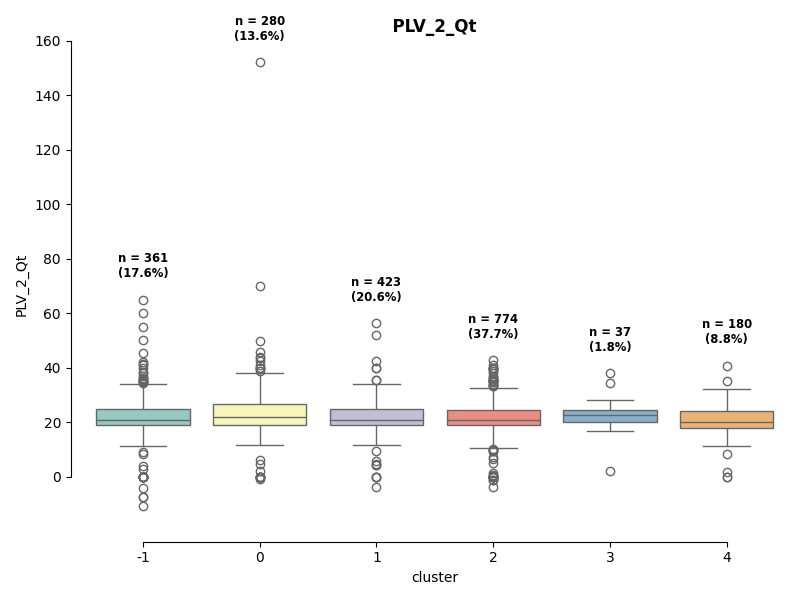
\includegraphics[width=0.75\textwidth]{clustering_pipeline/output/20250404_boxplot_PLV_2_Qt.png}
    \caption{PLV per quintal across clusters}
\end{figure}

\begin{figure}[h!]
    \centering
    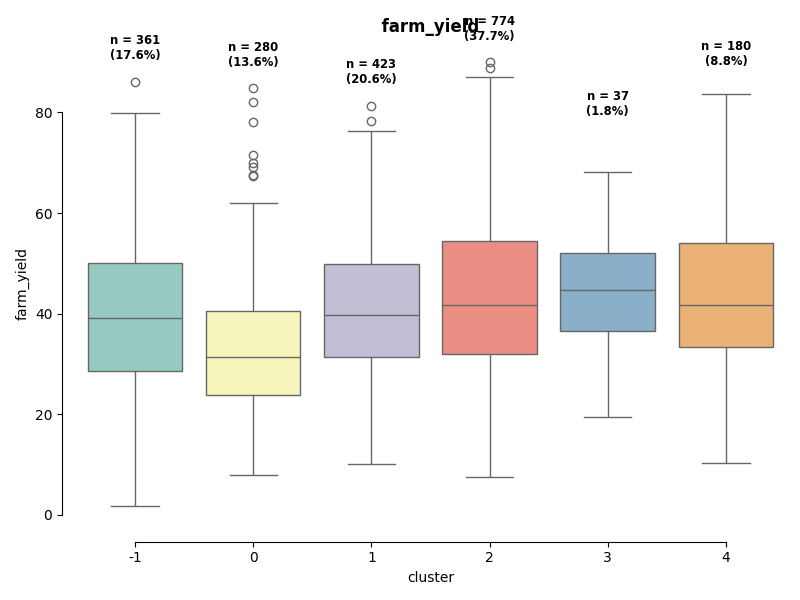
\includegraphics[width=0.75\textwidth]{clustering_pipeline/output/20250404_boxplot_farm_yield.png}
    \caption{Farm yield per hectare across clusters}
\end{figure}

\begin{figure}[h!]
    \centering
    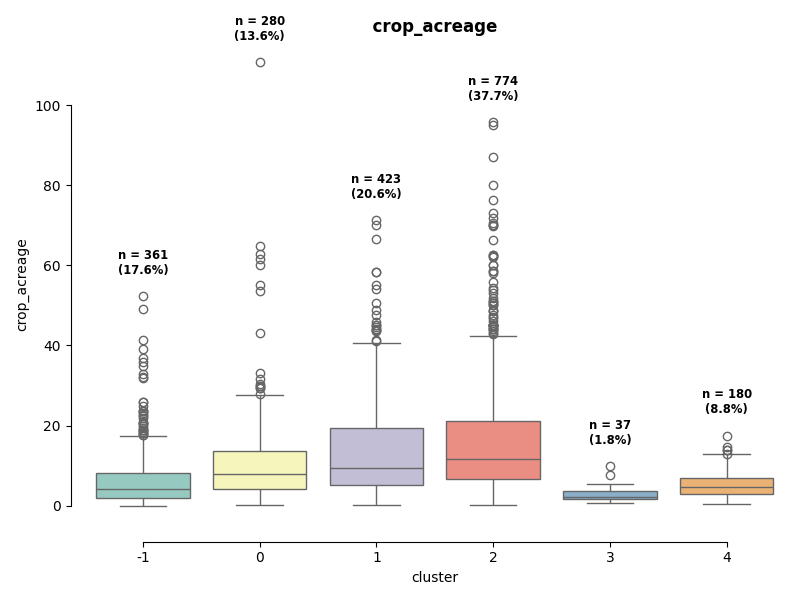
\includegraphics[width=0.75\textwidth]{clustering_pipeline/output/20250404_boxplot_crop_acreage.png}
    \caption{Crop acreage across clusters}
\end{figure}

\begin{figure}[h!]
    \centering
    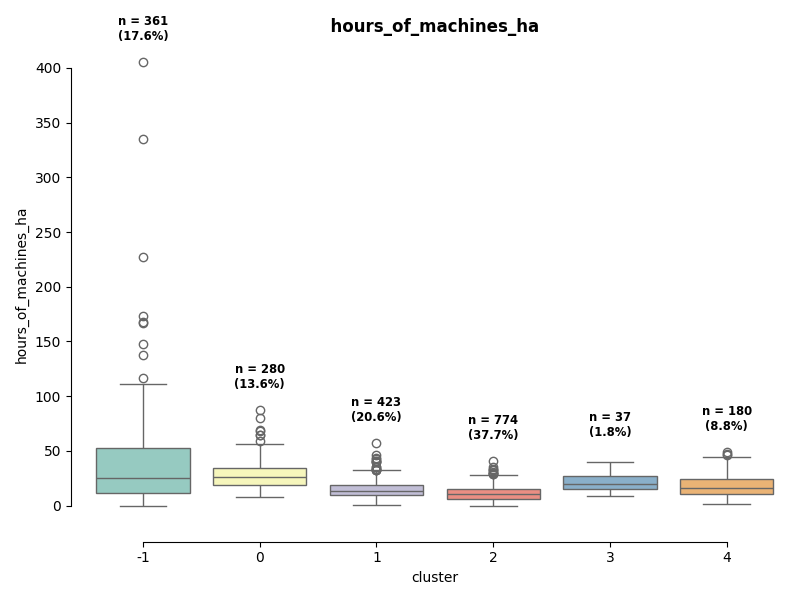
\includegraphics[width=0.75\textwidth]{clustering_pipeline/output/20250404_boxplot_hours_of_machines_ha.png}
    \caption{Machinery use per hectare across clusters}
\end{figure}

\begin{figure}[h!]
    \centering
    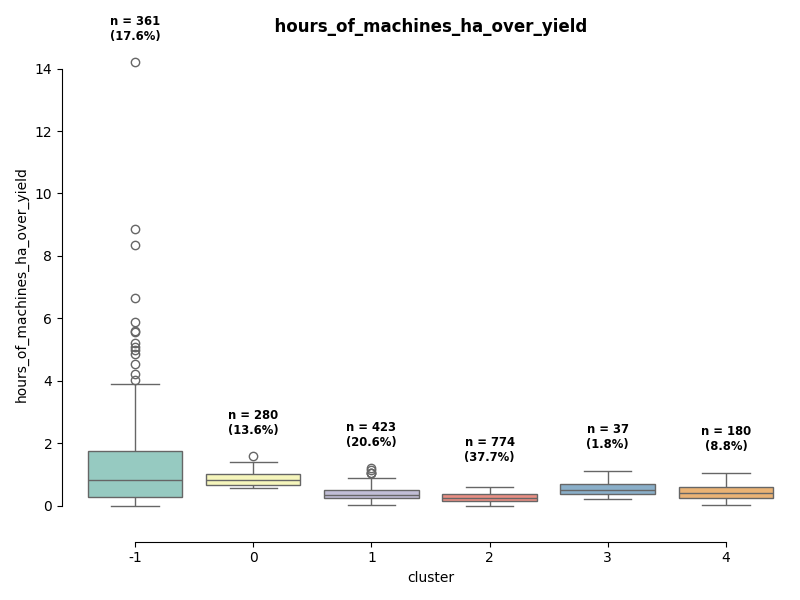
\includegraphics[width=0.75\textwidth]{clustering_pipeline/output/20250404_boxplot_hours_of_machines_ha_over_yield.png}
    \caption{Machinery use over yield across clusters}
\end{figure}

\begin{figure}[h!]
    \centering
    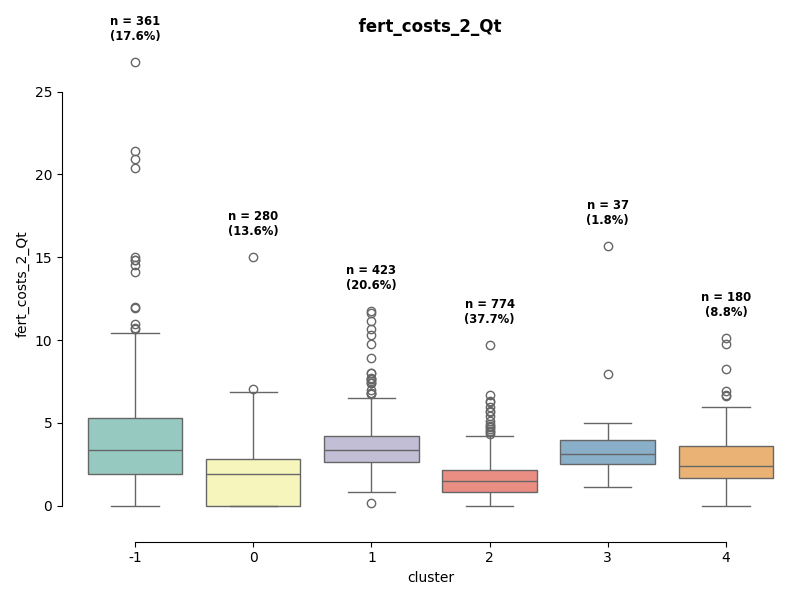
\includegraphics[width=0.75\textwidth]{clustering_pipeline/output/20250404_boxplot_fert_costs_2_Qt.png}
    \caption{Fertilizer costs per quintal across clusters}
\end{figure}

\begin{figure}[h!]
    \centering
    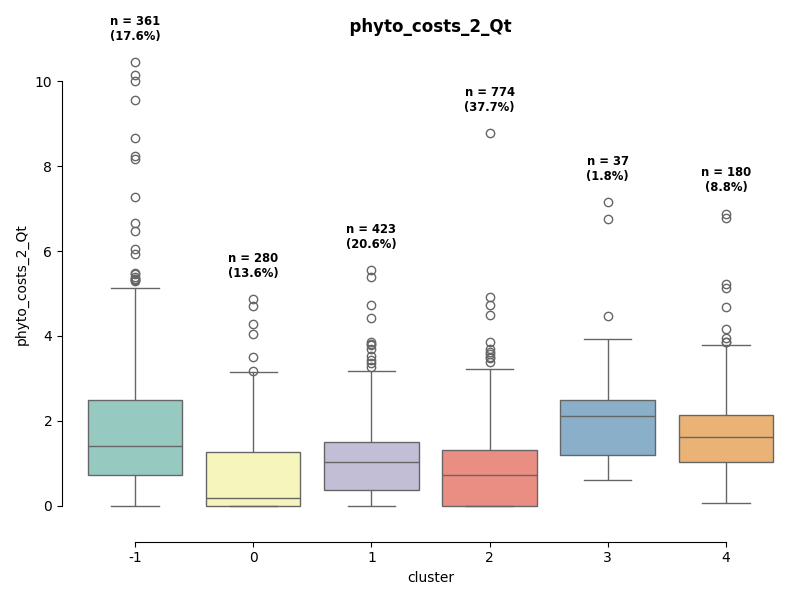
\includegraphics[width=0.75\textwidth]{clustering_pipeline/output/20250404_boxplot_phyto_costs_2_Qt.png}
    \caption{Phytosanitary costs per quintal across clusters}
\end{figure}

\begin{figure}[h!]
    \centering
    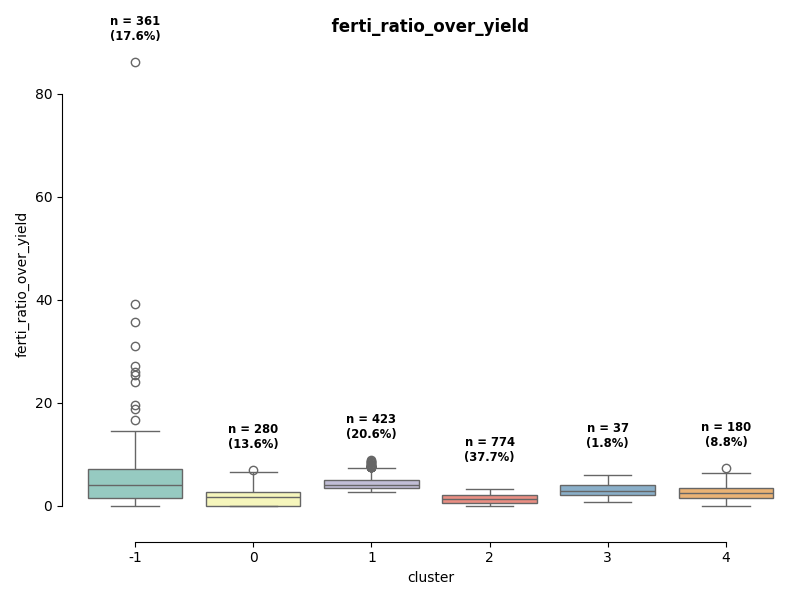
\includegraphics[width=0.75\textwidth]{clustering_pipeline/output/20250404_boxplot_ferti_ratio_over_yield.png}
    \caption{Fertilizer input ratio over yield across clusters}
\end{figure}

\begin{figure}[h!]
    \centering
    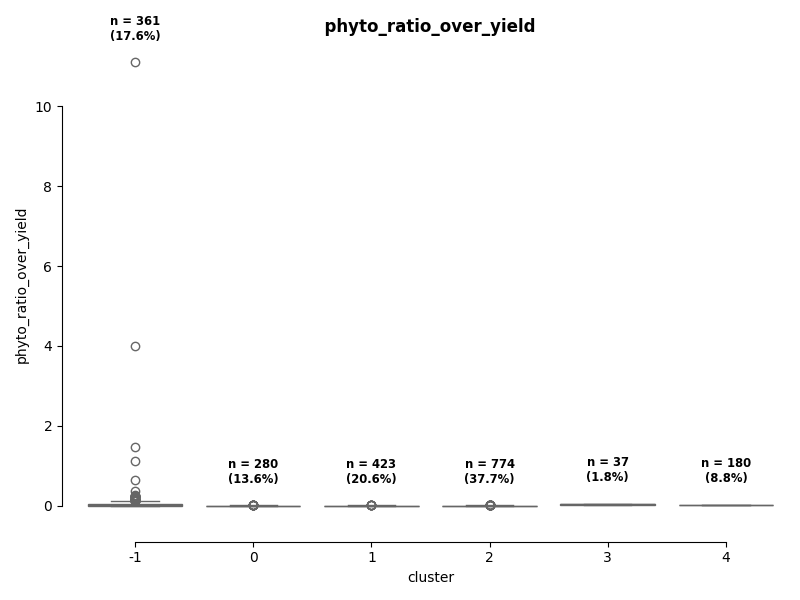
\includegraphics[width=0.75\textwidth]{clustering_pipeline/output/20250404_boxplot_phyto_ratio_over_yield.png}
    \caption{Phytosanitary input ratio over yield across clusters}
\end{figure}

\clearpage

\section{Conclusion}

The clustering procedure successfully segmented durum wheat farms into coherent groups based on resource use and productivity. The approach combines transparent preprocessing, robust outlier detection, and interpretable feature engineering. The resulting clusters offer a solid foundation for further simulation (e.g., agent-based models), targeted policy design, or exploratory analysis of input-output relationships in agriculture.

\end{document}
